\section{Objetivo}

El objetivo del proyecto es desarrollar un sistema automatizado y modular de un equipo carbonatador existente para la carbonatación de cerveza en barriles, capaz de garantizar calidad, precisión y consistencia en el proceso, bajo estándares industriales como ISA S88 \cite{BRAN}, y con capacidad de integración en sistemas de gestión mediante comunicación abierta.

\section{Equipo}
El equipo carbonatador a automatizar esta diseñado a medida para una planta de bajo nivel de producción. En la figura \ref{fig:p-and-id} se muestra un diagrama P\&ID con tags en formato IEC 81346-2 \cite{IEC}.

El sistema consiste en untanque de \(CO_{2}\) conectado a un barril de cerveza a través de la válvula solenoide QMB1. El barril se encuentra montado sobre una criba vibratoria que se acciona mediante el motor eléctrico MAA1. La presión interna del barril se mide con el transmisor BPA1.

\begin{figure}[H]
  \centering
  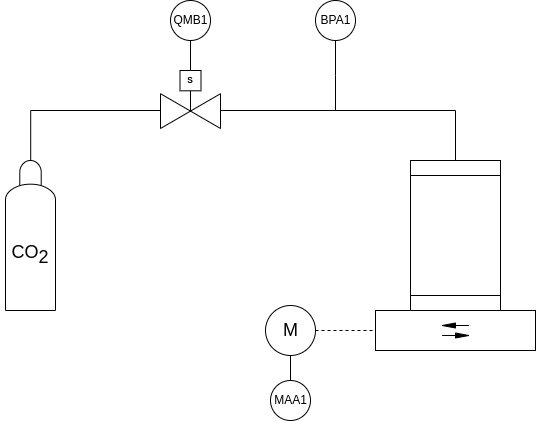
\includegraphics[width=0.75\textwidth]{introduccion-general/img/p-and-id.png}
  \caption{P\&ID del carbonatador}
  \label{fig:p-and-id}
\end{figure}

\section{Descripción del proceso}
En el proceso de elaboración de la cerveza una de las últimas etapas es la carbonatación, donde se incorpora dióxido de carbono a líquido para crear efervescencia, realzar el sabor, conservar la cerveza y otros propósitos. En el caso actual la carbonatación se realiza artificialmente mediante la incorporación forzada del gas.

El procedimiento se basa en la iteración de las siguientes dos fases, estructuradas según el patrón de diseño ISA S88 \cite{BRAN}:

\begin{itemize}
\item Inyección de CO2: Accionando la válvula solenoide (normalmente cerrada) (QMB1) se inyecta CO2 al barril de cerveza. La cantidad de gas inyectado se mide a través de la presión del barril (BPA1).
\item Disolución del CO2: Encendiendo la criba vibratoria (MAA1) se agita la cerveza y se favorece la disolución del CO2. El grado de disolución se mide indirectamente a través de la presión del barril (BPA1). A medida que el CO2 se diluye en la cerveza BPA1 decrece y se establece en un determinado valor. Se asume que se completó la disolución cuando dos muestras sucesivas de BPA1 con una separación de 1s difieren en menos de 10 mbar.
\end{itemize}

\subsection{Receta}
La receta que se requiere automatizar para lograr la carbonatación completa de un barril estándar se describe a continuación en pasos numerados y se muestra gráficamente en el diagrama de flujo de la figura \ref{fig:receta-de-carbonatacion}.

\begin{enumerate}
\item Se inyectan 3 bares de \(CO_{2}\) al barril accionando QMB1 hasta que \(BPA1 = 3\,bar\).
\item Se diluye el \(CO_{2}\) encendiendo la criba vibratoria. Si una vez diluido el gas se mide \(0.9\,bar < BPA1 < 1\,bar\) entonces se finaliza la receta con el barril correctamente carbonatado, sino si \(BPA1 < 0.9\,bar\) se pasa al paso 3.
\item Se inyectan 2 bares de \(CO_{2}\).
\item Se diluye el \(CO_{2}\) y si \(0.9\,bar < BPA1 < 1\,bar\) se finaliza satisfactoriamente la receta, sino si \(BPA1 < 0.9\,bar\) se pasa al paso 5.
\item Se inyecta 1 bar de \(CO_{2}\).
\item Se diluye el CO2 y si \(0.9\,bar < BPA1 < 1\,bar\) se finaliza satisfactoriamente la receta, sino si \(BPA1 < 0.9\,bar\) se repiten los pasos 5 y 6 indefinidamente.
\end{enumerate}

En los pasos 2, 4 y 6 la condición \(BPA1 > 1\,bar\) detiene la receta dado que no debería producirse si el sistema funciona adecuadamente. Se debe revisar el equipo.

\begin{figure}[H]
  \centering
  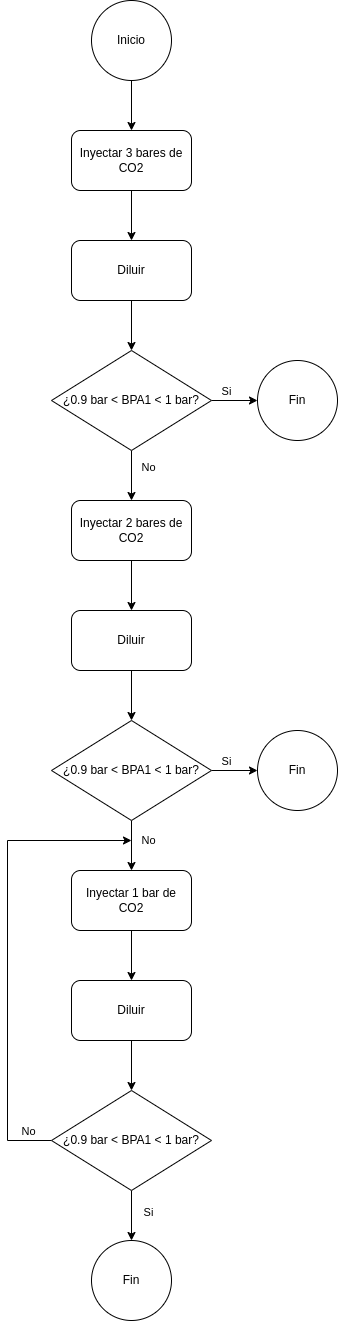
\includegraphics[height=\textheight]{introduccion-general/img/receta-de-carbonatacion.png}
  \caption{Diagrama de flujo de la receta de carbonatación.}
  \label{fig:receta-de-carbonatacion}
\end{figure}


\subsection{Interacción del operador}
La operación del sistema se basa en la ejecución de la receta de carbonatación, siguiendo el patrón de diseño de manufactura flexible ISA S88 \cite{BRAN}.

El operador controla el estado de la receta a través de los siguientes comandos:

\begin{itemize}
\item Start: inicia la receta.
\item Stop: detiene la receta.
\item Hold: pausa la receta.
\item Resume: reanuda la receta.
\item Reset: reinicia la receta.
\end{itemize}

Los comandos se encuentran ligados con los estados de la receta de acuerdo al diagrama de estados de la figura \ref{fig:estados-de-la-receta}.

\begin{figure}[H]
  \centering
  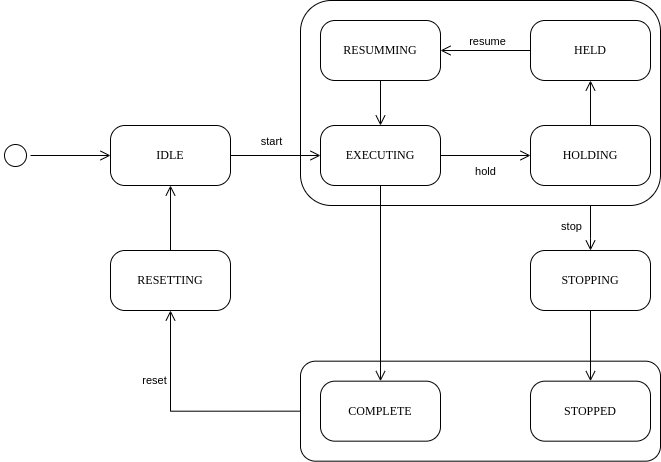
\includegraphics[width=\linewidth]{introduccion-general/img/recipe-state-diagram.png}
  \caption{Diagrama de estados de la ejecución de la receta de carbonatación.}
  \label{fig:estados-de-la-receta}
\end{figure}


\section{Arquitectura de control}
El sistema de automatización se basa en una arquitectura de control típica como se muestra en la figura \ref{fig:arquitectura-de-control}. Consta de un único controlador controlando el equipo físico, un HMI para operar y el soporte para una computadora de supervisión con la capacidad de monitorear el proceso, a través de una conexión serie o mediante un navegador web.

\begin{figure}[H]
  \centering
  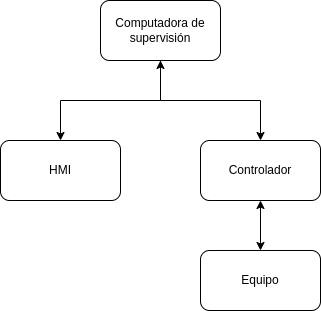
\includegraphics[width=0.5\linewidth]{introduccion-general/img/arquitectura-de-control.png}
  \caption{Arquitectura de control.}
  \label{fig:arquitectura-de-control}
\end{figure}

\section{Análisis de sistemas similares en el mercado}

En el mercado los carbonatadores que se venden son generalmente del tipo inline, para volúmenes altos de producción. El sistema a automatizar maneja volúmenes de producción bajos y por ende el carbonatador implementado opera directamente sobre los barriles. Sin embargo, se analizan tres sistemas de carbonatación comerciales para comparar las características de cada uno, en la tabla \ref{table:similares} se muestran los resultados de este análisis.

Los productos analizados se pueden encontrar en los siguientes enlaces:

\begin{itemize}
\item \href{https://www.probrew.com/products/procarb-mini/}{ProCarb™ Mini}
\item \href{https://foodandbeverage.pentair.com/en/products/pentair-carbonation-control-system-carbo-controller-ccr?utm_source=google&utm_medium=cpc&utm_term=HGB+Carbonator&utm_content=digital_ad&utm_campaign=CCR_awareness_2024}{Pentair Carbonation Control System}
\item \href{https://www.alfalaval.com/products/process-solutions/brewery-solutions/blending-modules/carboblend/}{Carboblend}
\end{itemize}

\begin{table}[H]
\centering
\begin{tabular}{|l|c|c|c|}
\hline
\rowcolor[HTML]{EFEFEF} 
\multicolumn{1}{|c|}{\cellcolor[HTML]{EFEFEF}\textbf{Característica}} & \textbf{ProCarb™ Mini} & \textbf{\begin{tabular}[c]{@{}c@{}}Pentair Carbonation\\ Control System\end{tabular}} & \textbf{Carboblend} \\ \hline
Automático                                                            & Si                     & Si                                                                                    & Si                  \\ \hline
HMI                                                                   & Si                     & Si                                                                                    & Si                  \\ \hline
Compacto                                                              & Si                     & Si                                                                                    & Si                  \\ \hline
\begin{tabular}[c]{@{}l@{}}Medición directa\\ de CO₂\end{tabular}     & Si                     & Si                                                                                    & Si                  \\ \hline
\begin{tabular}[c]{@{}l@{}}Comunicación\\ abierta\end{tabular}        & Si                     & Si                                                                                    & Si                  \\ \hline
\end{tabular}
\caption{Comparación de carbonatadores comerciales.}
\label{table:similares}
\end{table}

%%% Local Variables:
%%% mode: latex
%%% TeX-master: "../main"
%%% End:
